\chapter{Introduction}
\label{cha:introduction}

This chapter introduces the topic area of this thesis as well as the research questions
that this thesis focused on. The topic area of this thesis is introduced in Section \ref{sec:intro_topic}.
The research questions are posed in Section \ref{sec:rq}. Additionally,
this chapter describes the demonstrator project on which this thesis research
was conducted in Section \ref{sec:desc_demonstrator}. This is followed by an overview
of the structure of the thesis in Section \ref{sec:thesis_structure}. The chapter finishes
with a graphic overview of the relationship between the topics discussed in this thesis
in Section \ref{sec:content_overview}.

\section{Introduction to the Topic Area}
\label{sec:intro_topic}
% If the work is based on a concrete project scenario, this project scenario should already be introduced
% in this section at a high level of abstraction.

% TODO: Do
% Outline
% - Monitoring/DevOps
% - Decentralized Identity?
% - BestRentalPoC

Monitoring is a part of operating software.

\subsection*{Story of BestRentalPoC}

The following is the motivating story behind the demonstrator project BestRentalPoC
(BestRental Proof of Concept) that serves as a concrete project
on which the research of this thesis was conducted.

Alice is a customer of BestRental and has been renting cars from them.
However, every time she rented a car, she had to remember to bring her physical driving license.
Fortunately, DLAKa, the driving license authority in Karlsruhe, 
has introduced a digital driving license option. Alice heard the news and decided to go
to DLAKa to obtain her digital driving license. Bob, who works at DLAKa,
first checks that Alice's physical driving license is valid. Then, Bob fills out a digital form
using the data on Alice's physical driving license. Afterward, Alice scans the QR code on Bob's monitor
using her authenticator app and grants permission to create her digital driving license.
As a result, Alice now possesses a digital driving license in the wallet of her authenticator app.
Alice now can provide digital proof of her valid driving license to anyone who requests it.
Next, Alice rents a car from BestRental. But this time, she uses her digital driving license
to prove that she has a valid one. Once Alice opens the website of BestRental,
she will be prompted to present her digital driving license. Therefore, the website displays a QR Code,
which Alice scans with her authenticator app. Next, Alice confirms the presentation using
her authenticator app and decides what information gets shared. 
Finally, Alice has been verified on BestRental's website and can now rent a car. 
Alice provides the desired period and location for the car rental.
On the website, Alice can then browse and choose from available cars.
Once she has selected a car, BestRental will reserve the car for her.

% \subsection{Motivation BestRentalPoC}
% The company BestRental wants to develop a monitoring solution for its BestRentalPoC system
% to collect metrics that are meant to assist the company in operating the BestRentalPoC.
% The system will be operated by QA Engineers, system operators, and a project manager.
% Before developing the monitoring solution, the team tasked with developing the solution,
% interview the different roles to find out how they will use the solution
% and what their tasks and responsibilities are.
% QA Engineers are responsible for the reliability of BestRentalPoC.
% To ensure the reliability of the system, they want to know when requests to the system fail and
% trigger errors, so that they can fix them.
% For them to better understand errors, they want to know how often errors occur and from which services,
% inside of BestRentalPoC, they originate.
% The system operators run the BestRentalPoC. They need to make sure that at any point in time
% BestRentalPoC has enough instances of all of its services available to serve all incoming requests.
% Because BestRental wants to operate profitably, they can't just create as many instances as they like,
% and they need to shut down instances when they are not needed.
% To assist them with their task, they want to know how high the resource usage of each instance is
% and how many requests are coming into the system. The resources that they want to track for each
% instance are the instance's CPU and memory usage.
% The project manager's yearly bonus is tied to how profitable the BestRentalPoC operates.
% To ensure that he gets his bonus, the project manager wants to track the operating costs of the complete system.
% Additionally, he needs to how high the operating costs of each service are, so that he can
% allocate development time to increase the efficiency of a service, making it more profitable.
% After the interviews, the development notes that all types of users of the monitoring solution
% want to be able to do five different things.
% Firstly, they want to be able to create a dashboard for a metric that displays its current and historic values.
% When viewing a dashboard they also want to be able to run queries on the metric to, for example, get
% its value at a specific point in time.
% Because the users can't constantly watch all of their dashboards, they want to be able to create
% alerts for a metric that will be triggered when the metric exceeds a set value.
% When a metric exceeds a value set for an alert, the users want to receive the alert so that they can act on it.
% The developers also know that the solution needs to be able to do three main things to accomplish
% the requested features.
% Firstly, the solution needs to collect metrics from BestRentalPoC,
% it then needs to analyze the collected data, and lastly, it needs to conditionally send out alerts
% for metrics.

\section{Research Questions}
\label{sec:rq}
% The first research question should be superior to the following questions ''2 to n'' 
% and should be dealt with in the first content chapter which is Chapter 4.

% The second research question concerns the concrete software system which serves as a (first part of a)
% demonstrator for the overall research question. This software system will be developed in cooperation with
%  the project team (JuniorStudents) which is co-supervised by the author (SeniorStudent) of this thesis.
% Chapter 5 (Technical Foundation) introduces the existing preliminary work which particularly includes the already
% existing artifacts relevant for the software system to be developed. Chapter 6 (First Solution) describes the
% structured development approach of the software system (in the case of a microservice-based application,
% this is C\&M's microservice engineering approach).

% Research questions 3 to n should then be addressed in the following chapters.
% These research questions should be formulated in detail only AFTER clear answers to the second research question have
% been worked out since these results have a strong influence on the further alignment of the thesis.

% TODO: Do

\begin{enumerate}
	\item[RQ1:] How can monitoring be integrated into the UME (Unified Microservice Engineering) approach?
	Most research regarding DevOps-based software engineering processes and practices only focuses
	on the development and deployment part of DevOps while leaving out the operations.

	\item[RQ2:] How can the adapted UME approach be used to monitor BestRentalPoC?
	To prove the validity of the developed monitoring concept it should be applied
	to a project.
\end{enumerate}

\section{Description of the Demonstrator}
\label{sec:desc_demonstrator}
% The demonstrator should clarify the research questions introduced in the previous section on an appropriate conceptual level.
% The demonstrator introduces a practical example and shows a solution. In its first draft,
% it corresponds to the software system which is developed in cooperation with the co-supervised project team (JuniorStudents).

% TODO: Do

\section{Thesis Structure}
\label{sec:thesis_structure}

The following is a brief overview of the structure of this thesis.

\subsection*{Chapter 2: Foundations}

Chapter \ref{cha:foundations} contains a brief description of some general concepts
that are necessary for understanding this thesis. The concepts that are described
are decentralized identities, observability and monitoring, DevOps, and CI/CD.

\subsection*{Chapter 3: State of the Art}

Chapter \ref{cha:state_of_the_art} describes some of the research papers that were
used by this thesis. This chapter focuses on the influences of those papers on this
work and the question of whether or not they should be added to the Cooperation and Management
group's literature collection.

\subsection*{Chapter 4: Overall Concept of the Developed Solution}

% TODO:
Chapter \ref{cha:concept} develops the central idea of this thesis: The extension
of the UME approach with a monitoring concept. First, the UME approach,
which employs the DevOps concept, is described. This is followed by an analysis
of how monitoring is used in DevOps. Finally, the extension of the UME approach
by a monitoring concept is explained.

\subsection*{Chapter 5: Technical Foundations}

Chapter \ref{cha:technical_foundation} adds to Chapter \ref{cha:foundations}
by describing concepts that are necessary for the understanding of the solution
that was developed during this thesis but which differ from the concepts in Chapter \ref{cha:foundations}
by being of a more technical nature rather than general concepts.
The technical concepts described in this chapter are containerization, the tool ArgoCD,
and the tools used by the developed solution: Grafana, Prometheus, Grafana Mimir, and MinIO.

\subsection*{Chapter 6: Monitoring DLAKaApp}

Chapter \ref{cha:first_solution} contains the practical application of the concepts
developed in Chapter \ref{cha:concept}. The concept is applied to the microservice
DrivingLicenseManagement of BestRentalPoC. The chapter starts by extending the motivation
for BestRentalPoC to include the need for monitoring. Afterward, the development
of SPMonitor, a tool developed for monitoring BestRentalPoC, is described by going through
the different phases of software development one after another. First, the extended
motivation is analyzed from which use cases are derived that are used to
create requirements and capabilities for SPMonitor. After the analysis,
SPMonitor is designed. The design starts with an abstract software architecture
based on the general requirements for a monitoring tool described in Chapter \ref{cha:foundations}.
This is followed by an API specification for collecting metrics from the microservice DrivingLicenseManagement.
% TODO:
SPMonitor Client Lib
With the requirements and capabilities as a basis, the tools for SPMonitor are selected next.
Finally, the concrete software architecture of SPMonitor is designed.
The chapter concludes with the description of the implementation and deployment of SPMonitor.

\subsection*{Chapter 7: Organization of the Project Team}

Chapter \ref{cha:projektteam-arbeiten} describes the practical course
that accompanies the WASA2 lecture which is held by the Cooperation and Management group.
During his thesis, the author supervised P3 (project team 3) which was taking
part in the practical course. The tasks of P3 focused on the DevOps side of
BestRentalPoC.

\subsection*{Chapter 8: Contributions to the Practical Course Microservice2Go}

Chapter \ref{cha:m2go} describes the author's contributions to the planning
of a new practical course called Microservice2Go which will be offered by the
Cooperation and Management group alongside the WASA1 lecture, starting in the winter semester
2023/2024. The contributions were focused on the creation of exercises for the implementation part
in the third part of Microservice2Go called Microservice Engineering. This included
developing a microservice implementation which will be used as the template for the exercises.

\subsection*{Chapter 9: Summary and Outlook}

Chapter \ref{cha:outlook} contains the author's summary of this thesis
as well as an outlook on areas of research that require further attention in the future.

\subsection*{Chapter 10: Appendix}

Chapter \ref{cha:appendix} is the appendix to the main content of the thesis.
The appendix contains lecture slides that were developed by the author for the WASA2 lecture,
the summary of a so-called Snack and Learn seminar by iC Consult \cite{ICC-WEB},
and a copy of the best practices and guidelines that were developed by the author
for the Unified Microservice Engineering approach of the Cooperation and Management group.

\section{Content-related Overview}
\label{sec:content_overview}

% TODO: Check fits new figure

Figure \ref{fig:content_overview} illustrates the relationship between the topics
discussed in this thesis. A developer uses the UME (Unified Microservice Engineering) approach
by the C\&M (Cooperation \& Management) group for developing microservice-based software
that uses decentralized identities. Decentralized identities are a method of providing
credentials independent of a central authority based upon decentralization and cryptography.
The UME approach defines a process for developing microservice-based software
using the DevOps concept. The DevOps concept employs CI/CD (Continuous Integration/Continuous Deployment)
and containerization to increase the efficiency of software development.
CI/CD refers to the practice of continuously delivering new features of software instead
of only delivering the completed software. Containerization provides a method for
deploying software independent of its runtime environment which makes deployments
less complex and reproducible. This thesis extends the UME approach
with a monitoring concept for observing the developed software.
Monitoring collects pre-defined metrics from the software.
Metrics fall into the two categories of technical and business metrics.
Technical metrics relate to the operation and performance of the software.
Examples of technical metrics include the amount of memory used by the software.
Business metrics capture KPIs (Key Performance Indicators) that can be used
by a business to drive business decisions. An example of a business metric
is the usage of a feature.

\begin{figure}[h]
	\centering
	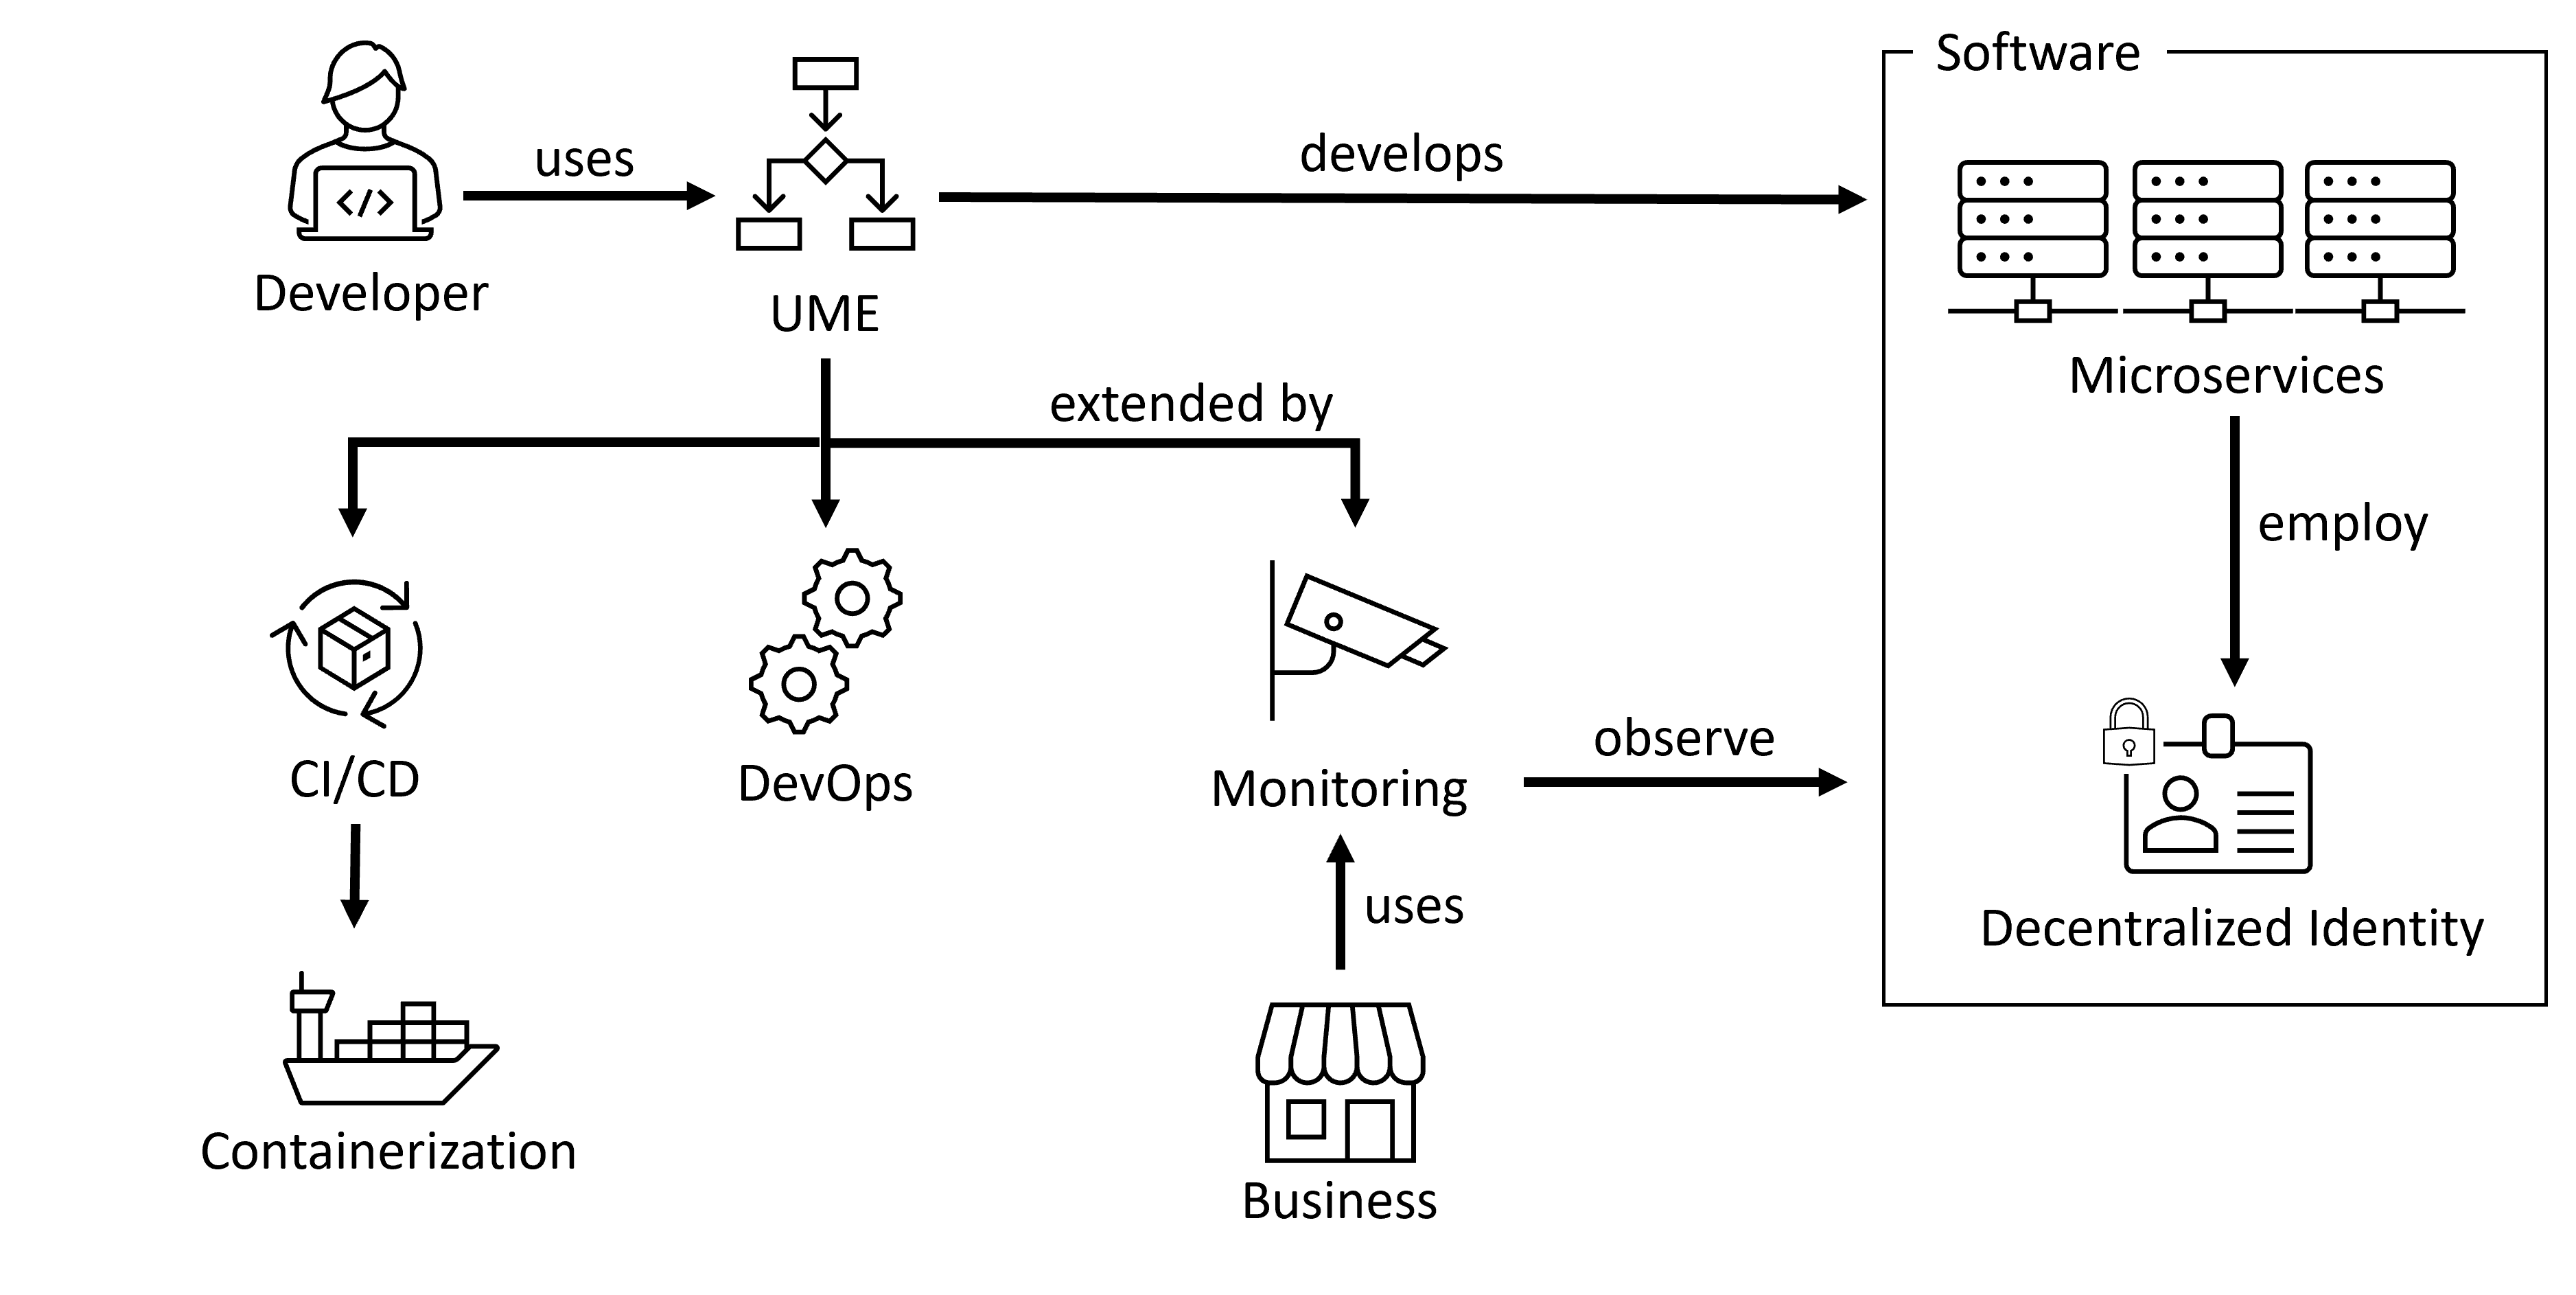
\includegraphics[width=\textwidth]{figures/content_overview.png}
	\caption{Content-related Overview}
	\label{fig:content_overview}
\end{figure}